\documentclass[11pt]{article}

\usepackage[paperwidth=200mm,paperheight=112.5mm,margin=7mm,top=6mm]{geometry}
\usepackage{amsmath,amssymb,graphicx,xcolor,enumitem,tikz}
\usetikzlibrary{arrows.meta}
\usepackage[T1]{fontenc}
\usepackage{lmodern}

\pagestyle{empty}
\setlength{\parindent}{0pt}
\setlist[itemize]{leftmargin=5mm,itemsep=4mm,topsep=2mm,parsep=0pt}
\graphicspath{{figures/}}

\newcommand{\slide}[1]{\clearpage{\LARGE\textbf{#1}}\par\vspace{2mm}}
% bullets left (38 %), figure right (60 %), figure as tall as the page allows
\newcommand{\twocol}[2]{%
  \begin{minipage}[t]{0.38\textwidth}\raggedright\large\vspace{4mm}#1\end{minipage}\hfill
  \begin{minipage}[t]{0.60\textwidth}\vspace{0pt}\centering
  \includegraphics[height=86mm]{#2}\end{minipage}}

\begin{document}

%======================================================================
\slide{Coulomb friction (simulated system only)}
\twocol{
\begin{itemize}
\item Per rail: $F = c_c \tanh(g\,v)$
\item Baseline model has no friction
\item $g = 1000$: at the rail velocities of the multisine, friction is fully Coulomb
\item At standstill the stage settles, no limit cycle
\end{itemize}
}{F3_friction_tanh.png}

%======================================================================
\slide{Measurement noise: where it enters}
\begin{center}
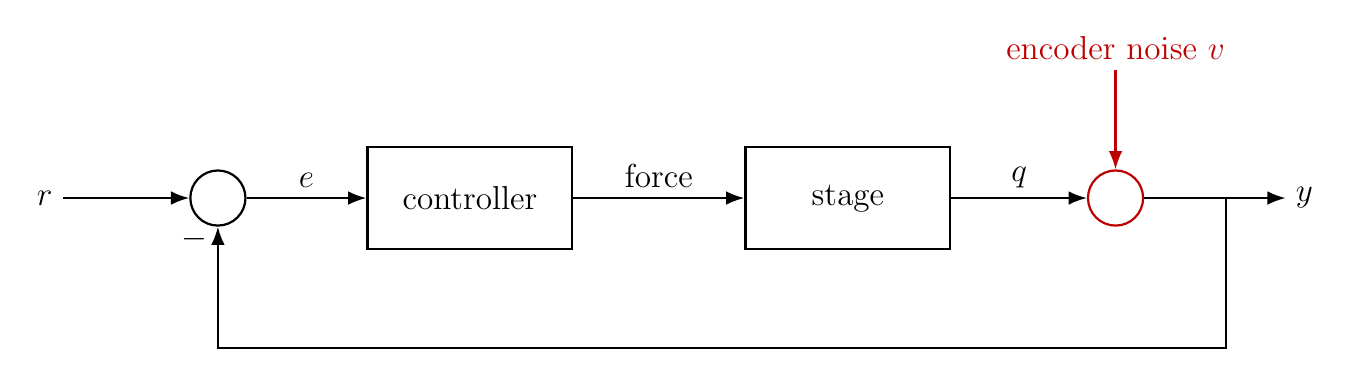
\begin{tikzpicture}[>=Latex, thick, font=\large,
    blk/.style={draw, minimum width=26mm, minimum height=13mm, align=center},
    sum/.style={draw, circle, minimum size=7mm, inner sep=0pt}]
  \node (r) at (0,0) {$r$};
  \node[sum] (s1) at (2.2,0) {};
  \node[blk] (K) at (5.4,0) {controller};
  \node[blk] (G) at (10.2,0) {stage};
  \node[sum, draw=red!75!black] (s2) at (13.6,0) {};
  \node (y) at (16.0,0) {$y$};
  \node[red!75!black] (v) at (13.6,1.9) {encoder noise $v$};
  \draw[->] (r) -- (s1);
  \draw[->] (s1) -- node[above] {$e$} (K);
  \draw[->] (K) -- node[above] {force} (G);
  \draw[->] (G) -- node[above] {$q$} (s2);
  \draw[->, red!75!black] (v) -- (s2);
  \draw[->] (s2) -- (y);
  \draw[->] (15.0,0) -- (15.0,-1.9) -| node[pos=0.95, left] {$-$} (s1);
\end{tikzpicture}
\end{center}
\vspace{4mm}
{\large
\begin{itemize}
\item $q$: true position; the encoder reads $y = q + v$
\item The controller only sees $y$, so it reacts to the noise
\item Servo error $e = r - y$: measured on the machine at standstill, this is our noise target
\item Goal: simulated $e$ at standstill $=$ measured $e$
\end{itemize}}

%======================================================================
\slide{Measurement noise: how it is shaped}
\twocol{
\begin{itemize}
\item The loop damps the noise at some frequencies and amplifies it at others
\item So per frequency we inject measured $\div$ what the loop lets through:
\[\Phi_v = \Phi_{\mathrm{meas}} / |S|^2\]
\item Below 50 Hz: not corrected (would need large slow noise)
\end{itemize}
}{F1b_noise_how.png}

%======================================================================
\slide{Measurement noise: result}
\twocol{
\begin{itemize}
\item Black: machine; blue: simulation
\item Above 50 Hz: match in shape and level
\item Below 50 Hz: slightly lower, $<1\,\%$ of the noise
\item Noise $\approx 10^{-8}$ m; signal-to-noise 58 to 79 dB
\end{itemize}
}{F1_noise_shape.png}

%======================================================================
\slide{Multisine band from the FRF}
\twocol{
\begin{itemize}
\item Top: truth vs baseline FRF; the gap is what the model misses (150 Hz dip, 264 Hz resonance)
\item Multisine goes where that gap is
\item Below 106 Hz (crossover): the motion references already excite it
\item Bottom: share of the gap from 106 Hz up; 90\,\% reached at 297 Hz
\item $\Rightarrow$ band 106 to 297 Hz (90\,\% is our choice)
\end{itemize}
}{F2_frf_band.png}

%======================================================================
\slide{Issue: absorber not learned above 230 Hz}
\twocol{
\begin{itemize}
\item Black: baseline error; orange: after training; the gap is what was learned
\item Below 230 Hz: 90\,\% removed
\item Above 230 Hz: only 22\,\%
\item Above 275 Hz: worse than the baseline
\item Same with another seed, with OBC, and with 4 added states
\end{itemize}
}{F4_absorber_issue.png}

%======================================================================
\slide{Why}
{\Large
\begin{itemize}
\item The model \textbf{can} hold the resonance (7$\times$ lower loss)
\item The loss \textbf{prefers} the resonance (truth 3.8$\times$ better)
\item But the static part of the network learns first and takes the absorber's place
\item Result: the added states stay static, no resonance
\item $\Rightarrow$ an optimisation problem, not data or model class
\end{itemize}
\vspace{6mm}
\textbf{Questions}
\begin{itemize}
\item How do we get the resonance into the added states?
\item Is it acceptable for the thesis if stated as a limitation?
\end{itemize}
}

\end{document}
